\documentclass[a4paper,10pt]{article}

\usepackage[utf8]{inputenc}
\usepackage[T1]{fontenc}
\usepackage{lmodern}
\usepackage{geometry}
\geometry{letterpaper}

\usepackage{doc}
\usepackage{url}

\usepackage{graphicx}
\usepackage{epstopdf}
\DeclareGraphicsRule{.tif}{png}{.png}{`convert #1 `dirname #1`/`basename #1 .tif`.png}


\geometry{hscale=0.85,vscale=0.85,centering}
\title{Protocole}
\author{Jean-Baptiste Dalle - Romain Gaborieau - Kevin Hivert - Alexis Braine}
\date{}

\begin{document}

\maketitle
\abstract{ Nous allons décrire dans la suite de ce document le protocole mis en place au sein de l'application de dessin collaboratif. Le protocole à été mis en place afin de permettre la connexion et la déconnexion d'un utilisateur, la transmission du dessin en temps réel entre tous les utilisateurs de l'application, la prise de contrôle sur le dessin en cours d'un utilisateur, etc... }


\subsection{Format des messages échangés.}
Afin de communiquer entre les clients et le serveurs nous avons définis un format précis de messages à envoyer qui permettra de savoir qui a envoyé le message d'une part et de faire passer une commande / une instructions et éventuellement (suivant le type de la commande) des paramètres ou des informations complémentaires. \\ \\

%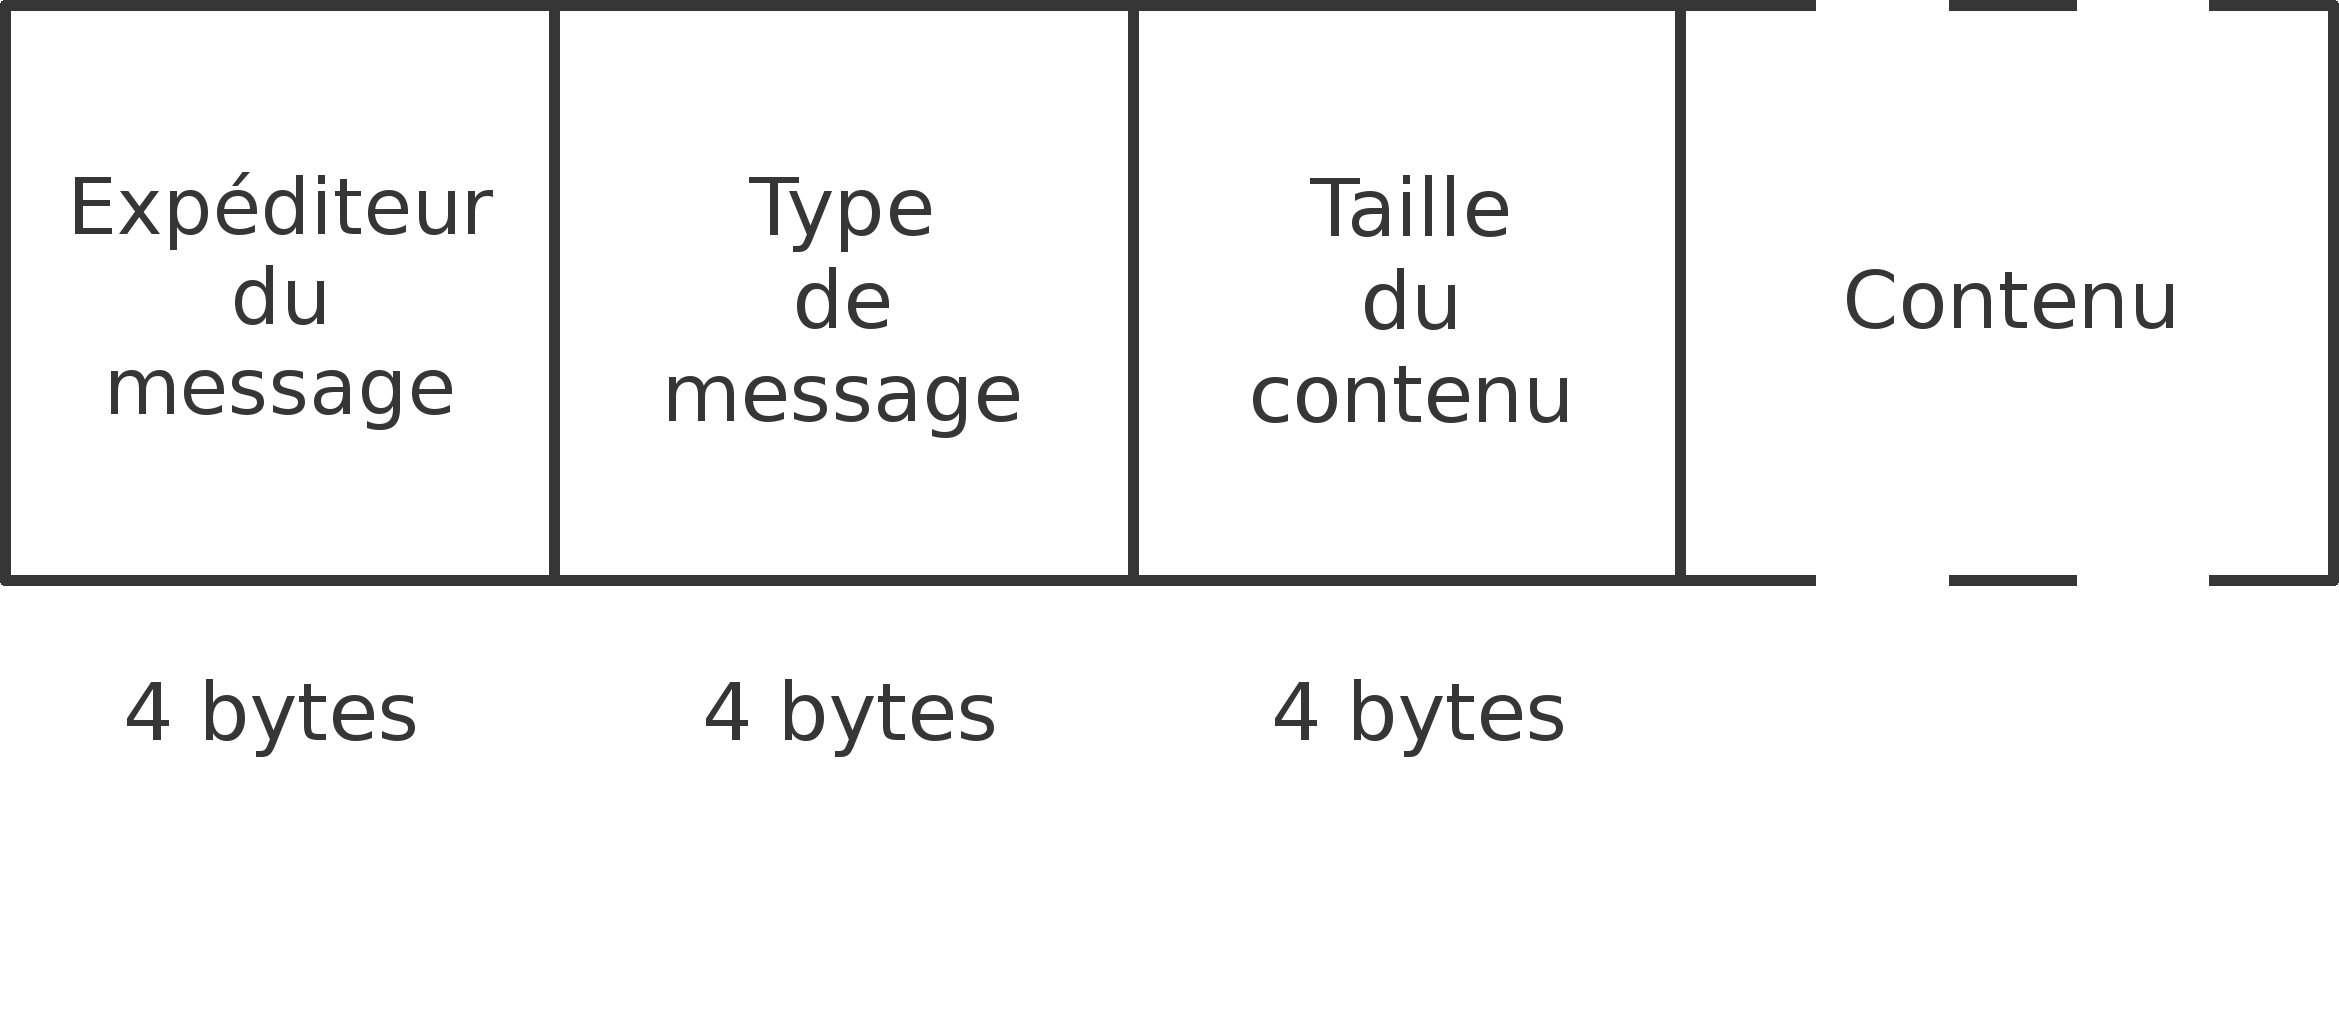
\includegraphics[scale=0.5]{message.png}

\paragraph{}Les messages sont donc constitués de quatre parties : 
\begin{itemize}
\item[1] L'adresse du destinataire, sur 4 octets.
\item[2] Le type de la commande, sur 4 octets également.
\item[3] La taille du contenu du message stocké sur 4 octets.
\item[4] Enfin, le contenu du message.
\end{itemize}


\paragraph{}\textit{Du point de programmation les messages sont stocké dans des byte[] et non pas de char[], car en Java un char est stocké sur 2 octets au lieu de 1. Pour des raisons de compatibilité avec d'autres langages nous avons donc pris la précaution de stocker les caractères des messages transmis sur des octets.}

\paragraph{}Le format ainsi construit des message nous permet donc aisément de savoir qui à envoyé le message et donc de lui répondre, d'envoyer des informations au client ou au serveur. Cela permet aussi au serveur d'envoyer des ordres aux clients (Le serveur peut indiquer à tout les clients que c'est au tour de tel client de prendre le contrôle du dessin), ainsi qu'au client d'envoyer des demandes au serveur (Le client peut demander à prendre la main par exemple).

\subsection{Types de messages échangés.}
\paragraph{}Afin de faire fonctionner notre application nous avons mis en place 13 commandes différentes qui vont être échangées entre les clients et la serveur.


\paragraph{}\begin{itemize}
\item CONNECT : Cette commande est utilisée par le client pour demander une connexion auprès du serveur. Cette commande est utilisée avec comme contenu de message le pseudo désiré par le client. Cette commande attend en retour, comme réponse soit la commande ACCEPT, soit la commande DENY que nous verons plus tard.

\item DISCONNECT : Cette commande est utilisée par le client pour se déconnecter. La commande n'attend rien en retour, le serveur en recevant le message retire le client de sa liste.

\item ACCEPT : Cette commande est envoyé par le serveur au client pour informer que le pseudo demander par le client et valide et que la connexion est accepté. Cette commande est aussi utilisé par le client pour informer le serveur qu'il est près à recevoir le dessin stocké sur le serveur.

\item DENY : Cette commande est envoyé par le serveur dans le cas où le pseudo demander par le client est déjà utilisé. Le client doit alors demander un autre pseudo.

\item  REQUEST$\_$CTRL : Il s'agit de la commande utilisé par les clients pour demander le contrôle du dessin.  Lorsqu'un client demande à prendre le contrôle du dessin le serveur l'ajoute à une liste d'attente, le client en tête de la liste obtient le contrôle pendant 30 secondes. A la fin du temps imparti, le client qui avait le contrôle est éliminé de la liste et on passe au client suivant, le client qui avait le contrôle doit donc redemander le contrôle pour être ré-inséré en fin de liste d'attente.

\item GIVE$\_$CTRL : Cette commande est utilisée par le serveur pour indiquer aux clients, qui prend le contrôle. 

\item LEAVE$\_$CTRL : Cette commande est envoyée du serveur au client qui a la main, afin qu'il la relâche,

\item SUBMIT : Cette commande est envoyé à chaque fois que le dessin est modifié. Le client qui a la main, l'envoie au serveur quand il fait une modification. Le contenu du message joint avec la commande est le contenu du dessin, c'est à dire le document SVG servant à le stocker.

\item UPDATE : Cette commande est renvoyé par le serveur à tous les client après qu'il ait reçu une modification du dessin de la part du client qui a le contrôle du dessin. Comme pour la commande SUBMIT, le contenu du message est le document SVG qui stocke le dessin.
On envoie également cette commande lorsque le client se connecte et qu'il a indiqué avec la commande ACCEPT, qu'il était près à recevoir le dessin.

\item GET$\_$USERS : Les clients utilisent cette commande pour demander la liste des utilisateurs connectés. Nous n'utilisons actuellement pas cette commande dans notre application, mais elle pourrait très bien servir pour afficher la liste complète des utilisateurs à chaque client et pourrait permettre d'ajouter un tchat à notre application de dessin.

\item LIST$\_$USERS : La commande devait servir de réponse à GET$\_$USERS, le contenu du message contient la liste des utilisateurs dans la même room que le client qui reçoit le message.

\item LIST$\_$ROOMS : Cette commande est envoyée par le serveur au client demandant une connexion afin qu'il puisse choisir une room dans la liste. Une room représentant un serveur avec un dessin différent stocké sur chaque room.
Nous n'avons cependant pas eu le temps d'implémenter complètement cette fonctionnalité à notre application, nous n'utilisons donc qu'une seule et unique room.

\item JOIN$\_$ROOM : Cette commande est utilisé par le client pour indiquer au serveur quelle room il veut rejoindre, et donc sur quel dessin il veut travailler.
\end{itemize}

\subsection{Déroulement du protocole}
\paragraph{}Nous allons maintenant suivre dans cette partie le déroulement du protocole depuis la connexion d'un client jusqu'à la modification du dessin et les répercutions de cette modification sur les autres clients.

\paragraph{}Ce protocole peut se diviser en 3 phases : 
\begin{itemize}
	\item[1] La connexion proprement dite, où le client choisit son pseudonyme (ainsi que sa room si cette fonctionnalité est implémentée
	\item[2] La communication de données, que l'on peut séparer en 2 catégories :
	\begin{itemize}
		\item[a] La réception de données, pour tous les clients
		\item[b] L'envoi de mises à jours concernant le dessin, fait seulement par le client ayant la main
	\end{itemize}
	\item[3] La déconnexion du client, annoncée par un message spécifique
\end{itemize}


\textit{Dans ce chapitre, les messages seront décrits sous la forme [ expéditeur ; type ; contenu ] pour plus de lisibilité}

\subsubsection{Connexion}
On suppose que le client A veut se connecter à un serveur, sur lequel sont déjà les clients B et C.
\begin{itemize}
	\item[1] A envoie une demande de connexion au serveur, du type [ A ; CONNECT ; mon\_pseudo ]
	\item[2] Si le serveur ne comporte aucun client portant ce pseudo, il renvoie [ SERVER ; ACCEPT ; ] \\
	Sinon, il renvoie [ SERVER ; DENY ; ] et le client recommence l'étape 1
	\item[3] Comme le client prend un certain temps (variable selon la machine employée) pour préparer son interface, le serveur attends de lui un message de confirmation [ A ; ACCEPT ; ], qui indiquera que la transmission des données de dessin peut commencer
\end{itemize}

\paragraph{}Lorsqu'un client démarre l'application, il se trouve face à une boite de dialogue lui demandant le pseudo qu'il veut utiliser, ainsi que l'adresse du serveur. On ouvre alors une connexion entre le serveur et le client en premier lieu.

Ensuite on test si le pseudo demandé par le client est valide, ceci ce fait en envoyant un message avec la commande CONNECT et le pseudo désiré par le client au serveur. Le serveur test alors l'unicité du pseudonyme, et renvoie le message approprié.

La connexion entre le serveur et le client étant engagé avant même que le client est réellement démarré l'application de dessin, si le client s'arrête (en fermant la fenêtre de connexion) alors le message DISCONNECT est envoyé au serveur qui s'occupe de rompre la connexion.


\paragraph{}Le serveur se met ensuite en attente d'un message du client l'informant qu'il est prêt à recevoir le dessin, l'application pouvant mettre du temps à charger nous devons être sur que tout soit en place pour recevoir et afficher le dessin.

Quand le client à chargé tout ses composants il envoie au serveur le message avec la commande ACCEPT, celui si répond alors en envoyant un message avec la commande UPDATE et comme contenu le dessin SVG qu'il stocke à ce moment. Le client est maintenant correctement connecté et peut alors afficher le dessin, et recevoir les futurs modifications ou demander à prendre la main, etc

\subsubsection{Processus de prise de main}
Afin de pouvoir modifier le dessin, le client A doit avoir la main sur son serveur. Pour cela, il va la demander en envoyant un message [ A ; REQUEST\_CTRL ; ].

Le serveur recevra cette requête et ajoutera donc A à la fin de la file d'attente pour la prise de main (ou lui donnera la main immédiatement si la file est vide). Lorsque le client ayant la main la rend, le client suivant est pris dans la file d'attente, et reçoit la main pour un temps défini (ici, 30 secondes). Le serveur fait alors savoir au client A que celui-ci a la main par le message [ SERVER ; GIVE\_CTRL ; A ]. Ce message est aussi transmis à tous les autres clients afin que ceux-ci sachent qui a la main.

Après 30 secondes, le serveur fait savoir au client A que son temps est écoulé, et fait savoir par la même occasion aux autres clients que A n'a plus la main par le message [ SERVER ; LEAVE\_CTRL ; A ].

\subsubsection{Envoi de données par le clients ayant la main}
Lorsque le client A a la main, il va donc renvoyer la totalité du dessin à chaque modification effectuée (souris relachée pour la création de forme, bouton cliqué pour le redimensionnement/déplacement). Bien que ce soit plus coûteux, cette technique permet d'éviter beaucoup de bugs de synchronisation entre le client et le serveur. Ces messages se présenteront sous la forme [ A ; SUBMIT ; nouveau\_dessin ]

\subsubsection{Transmission de l'image du serveur au client}
Le serveur va ensuite transmettre l'image mise à jour à tous les clients (c'est aussi par ce procédé que le client reçoit l'image après sa connexion). De la même façon, pour éviter des problèmes de synchronisation, le dessin est transmis en entier à chaque fois. Le message sera [ SERVER ; UPDATE ; nouveau\_dessin ].

\subsubsection{Déconnexion}
Lorsque le client A souhaite se déconnecter, il prévient d'abord le serveur par un message [ A ; DISCONNECT ; ], pour éviter que le serveur continue d'écouter sur un socket "vide". Il peut ensuite se déconnecter sans risque : en effet, l'emploi du protocole TCP pour acheminer les messages permet d'être sûr que le serveur a bien reçu cette annonce de déconnexion.

\end{document}